\section{Die Revolution von 1848}
\label{sec:rev-1848}
\index{Revolution!März 1848}

\subsection{Kampf zwischen Liberalismus und Restauration -- Der Weg
zur Revolution}
\label{ssc:kampf-lib-res}

\begin{aufgabe}
Weisen Sie nach, dass die Entwicklung im Zeitraum zwischen 1815 und
1848 in eine Revolution führen musste!
\end{aufgabe}

\begin{figure}
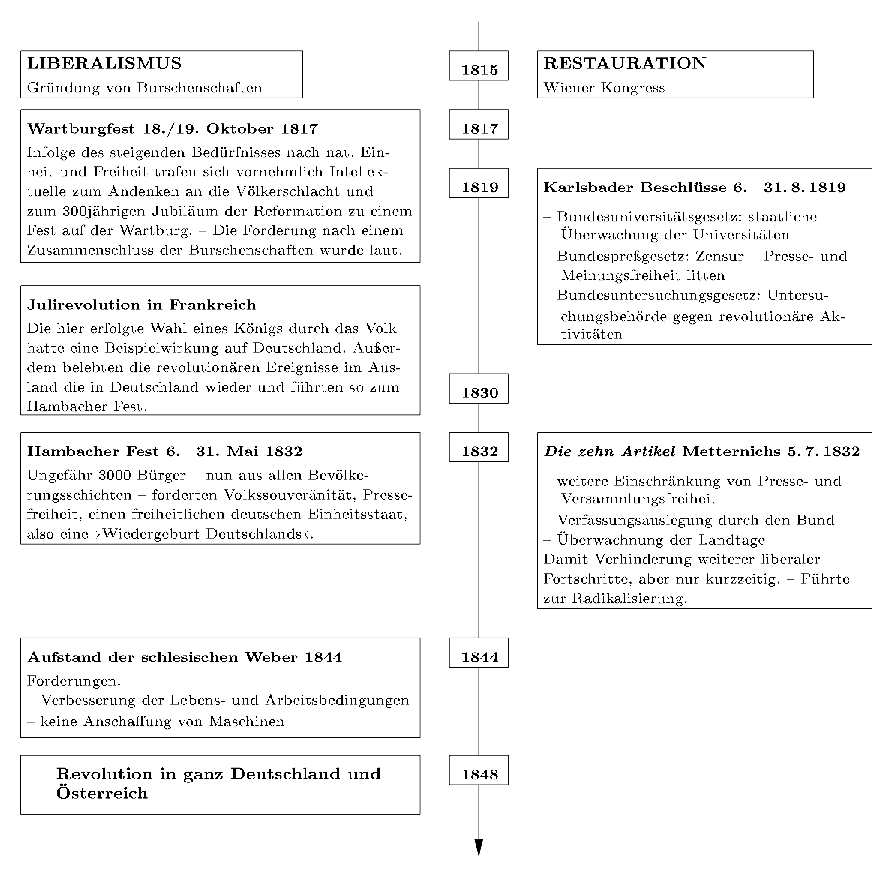
\includegraphics[width=\textwidth]{kampf-lib-rest.eps}
\caption{Das Ringen zwischen Liberalismus und Restauration}
\label{pic:kampf-lib-rest}
\end{figure}

Abbildung \ref{pic:kampf-lib-rest}\footnote{Die \ges{Zehn Artikel}
\Nam{Metternich, Klemens Wenzel Lothar von}{Metternichs} sind in
\cite{ZehnArt} zu finden, weitere Literatur in
\cite[106]{braunesGeschichts}. Die Quellen zu den übrigen Ereignissen
sind mir nicht bekannt.} zeigt die wichtigsten Ereignisse auf dem Weg
zur Revolution von 1848. Man erkennt, dass die Intensität von
antirestaurativen und restaurativen Maßnahmen immer weiter zunahm.
Weiter befeuert wurde die entwicklung durch die sich in Folge der
Industriellen Revolution verschärfenden soziale Lage.

%%%%%%%%%%%%%%%%%%%%%%%%%%%%%%%%%%%%%%%%%%%%%%%%%%%%%%%%%%%%%%%%%%%%%%

\subsection{Ursachenfeld}

\renewcommand*{\arraystretch}{1.5}
\newcolumntype{Y}{>{\setlength{\hsize}{0.55\hsize}\raggedleft}X}
\newcolumntype{Z}{>{\setlength{\hsize}{0.45\hsize}\raggedright}X}
\begin{tabularx}{\textwidth}{Y@{\quad$\lightning$\quad}Z}
restaurative Bewegung   & liberale Bewegung     \\
Absolutismus            & Aufklärung            \\
Industrielle Revolution -- Reichtum
                        & soziale Mißstände -- Armut    \\
territorialstaatlicher Absolutismus
                        & Einheitsbestrebungen
\end{tabularx}

%%%%%%%%%%%%%%%%%%%%%%%%%%%%%%%%%%%%%%%%%%%%%%%%%%%%%%%%%%%%%%%%%%%%%%

\subsection{Anlass}

Begünstigt durch die \dat{Krisenjahre 1847/48} in Frankreich mit
Missernten und Hungerunruhen kam es dort zur
\emph{Februarrevolution}\index{Februarrevolution}. Die Ereignisse in
Frankreich nahm man sich dann in Deutschland zum Vorbild und begann
die Revolution, die schon lange auf ihren Ausbruch gewartet hatte.
\mar{Germania und Bedeutung/Entwicklung von Symbolen.}

%%%%%%%%%%%%%%%%%%%%%%%%%%%%%%%%%%%%%%%%%%%%%%%%%%%%%%%%%%%%%%%%%%%%%%

\subsection{Verlauf}

\begin{figure}
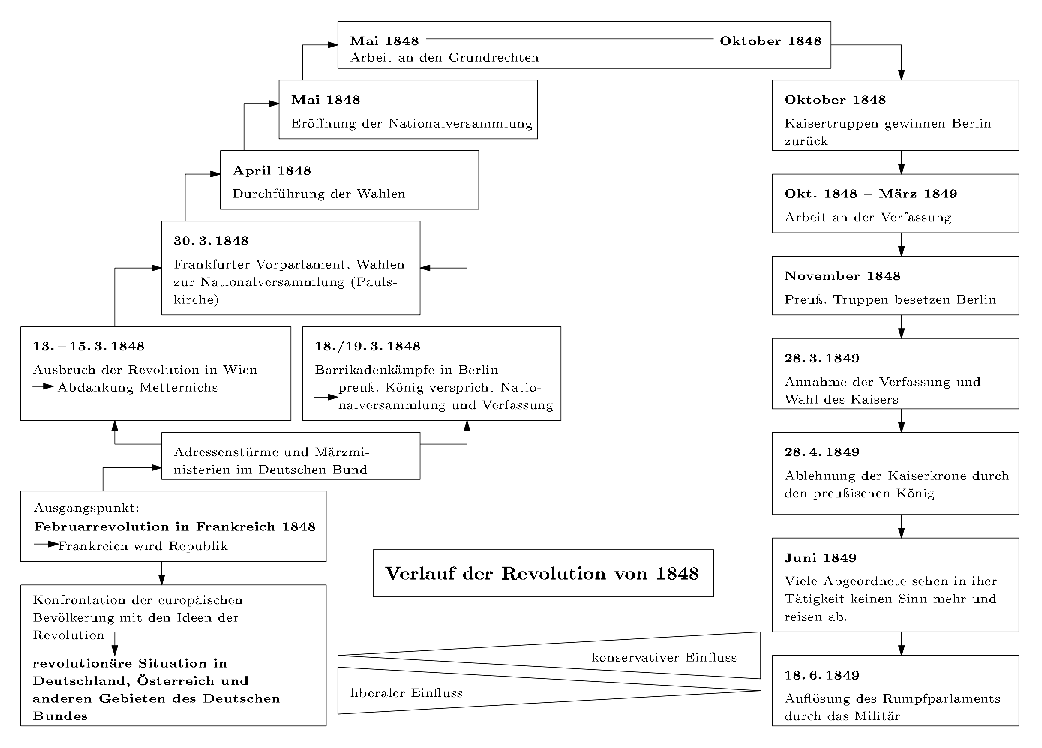
\includegraphics[height=\textwidth, angle=90]{verlauf-rev.eps}
\caption{Verlauf der Revolution von 1848}
\label{pic:verlauf-rev}
\end{figure}

Abbildung \ref{pic:verlauf-rev} bietet einen Überblick über den
Verlauf der Revolution. Diesen kann man in drei Etappen einteilen:
\mar{Richtige Benennung der Phasen?}

Die erste Phase war von kämpferischen Handlungen geprägt. Mit dem
Zusammentritt des \emph{Frankfurter Vorparlaments}
\index{Vorparlament!Frankfurt} begann eine Phase der Machtfestigung.
Der Niedergang setzte in der sehr langen Zeit der \emph{Arbeit an den
Grundrechten} ein. Diese Verzögerung der Vorgänge war nämlich einer
der Gründe für das Scheitern der Revolution: Durch die Uneinigkeit und
die fehlende parlamentarische Erfahrung, dauerte die Komprmissfindung
sehr lange. Das entstehende Machtvakuum nutzten die restaurativen
Kräfte für die Reaktion.

%%%%%%%%%%%%%%%%%%%%%%%%%%%%%%%%%%%%%%%%%%%%%%%%%%%%%%%%%%%%%%%%%%%%%%

\subsection{Verfassungsarbeit}

\begin{aufgabe}
Erläutern Sie die wesentlichen Aufgaben, die die
Paulskirchenversammlung zu lösen hatten und bilanzieren Sie die
jeweilige Lösung! 
\end{aufgabe}

\subsubsection{Parlament}

Das Parlament tagte in der runden
\Ort{Paulskirche!Frankfurt}{Frankfurter Paulskirche}\index{Frankfurt}.
Die 812 Männer unter dem Vorsitz des Liberalen \Nam{Gagern, Heinrich
von}{Heinrich von Gagern} waren hauptsächlich Bildungsbürger und
keinerlei Arbeiter. Man nannte die Versammlung daher auch
\jar{Parlament der Intellektuellen}.


\subsubsection{Grundrechte}
\index{Grundrechte}

Der erste Schwerpunkt der zukünftigten Verfassung für Deutschland
waren die Grundrechte. Auf Basis der Forderungen der Liberalen wurde
so ein umfangreicher Grundrechtskatalog beschlossen und im
\ort{Dezember 1848 angenommen}.


\subsubsection{Grenzen}

Eine sehr umstrittene Frage, die die Verhandlungen stark in die Länge
zog waren auch die zukünftigen Grenzen Deutschlands. Die
\emph{Großdeutsche Lösung} \index{Großdeutsche Lösung} sah neben den
deutschen Ländern die Einbeziehung der deutschsprachigen Teile
Österreichs vor. Diese wurde von vielen als die beste Variante
angesehen.

Österreich wollte jedoch sein gesamtes Staatsgebiet
einbringen, um als Gegengewicht zu Preußen auftreten zu können. Die
sogenannte \emph{Großösterreichische Lösung}
\index{Großösterreichische Lösung} war jedoch auch nicht möglich, da
man ein \emph{Deutsches} Reich wollte.

So fand man schließlich den Kompriss, Österreich ganz auszuschließen,
indem man zur \emph{Kleindeutschen Lösung} \index{Kleindeutschen
Lösung} gelangte.


\subsubsection{Staat}

Auch der \emph{Staatsaufbau} war Gegenstand langer Diskussionen zwischen
Demokraten, die eine Republik wollten und Liberalen, die eine
konstitutionelle Monarchie befürworteten. Das Ergebnis war das
System, welches Abbildung \ref{pic:verf-paulsk}\mar{Scan aus braunem
Geschichtsbuch S. 128 einfügen.} zeigt. \mar{Kriterien für
Verfassungsbewertung: Machtballungen, Rolle des Volkes, Verhältnis der
Organe} Es fallen dabei besonders die weitgreifenden Befugnisse des
Kaisers, die nicht mit dem Prinzip der Gewaltenteilung zu vereinbaren
sind, die freien Gerichte und der ausgeprägte Föderalismus auf.

Das Paulskirchenparlament musste auch die Entscheidung über das
künftige \emph{Staatsoberhaupt} fällen. Man wählte den Preußenkönig
\nam{Friedrich Wilhelm \Rm{4}}. Dieser lehnte allerdings ab, da er die
Krone nur \jar{aus den Händen eines deutschen Fürsten} empfangen
wollte. Die Verfassung war damit gescheitert.

%%%%%%%%%%%%%%%%%%%%%%%%%%%%%%%%%%%%%%%%%%%%%%%%%%%%%%%%%%%%%%%%%%%%%%

\mar{Das nennt sich wohl Bilanz.}
\subsection{Leistungen und Grenzen}

\begin{aufgabe}
Erörtern Sie die Darstellung, indem Sie die Hauptaussagen zur Wertung
der Revolution herausarbeiten, begründen, warum die Revolution trotz
iher fortschrittlichen Ideen scheiterte und sich zum Begriff des
epochalen Einschnitts für das Jahr 1848 positionieren!
\end{aufgabe}

\mar{?}
\begin{itemize}
\item Wertung der Verfassung
\item Nachweis des fraktionellen Kompromisses 
\end{itemize}

\subsubsection[Gründe des Scheiterns]{Gründe des
Scheiterns\mycite[138\,--\,140]{braunesGeschichts}}

\begin{itemize}
\item keine Hauptstadt $\rightarrow$ Polyzentrismus (viele kleine
Revolutionsherde)
\item keine parlamentarischen Machtmittel (Geld, Truppen)
\item Furcht vor Weiterführung der Revolution in soziale Revolution
\item Macht der Einzelmonarchen
\item Uneinigkeit durch unterschiedliche Ziele (auch sozial)
\item Unterschätzung der konservativen Kräfte
\end{itemize}


\subsubsection[Bedeutung für die deutsche Geschichte]{Bedeutung für
die deutsche Geschichte\mycite[140/141]{braunesGeschichts}}

\begin{itemize}
\item zuerst starke Zurückdrängung der liberalen Bewegung
\item Bestehenbleiben des Verfassungsstaates (konstitutionelle
Monarchien) in den deutschen Ländern außer Österreich
\item Abschaffung der Zensur

\item keine weitere Infragestellung von
\begin{itemize}
\item Bauernbefreiung
\item Ende der adeligen Patrimonialgerichtsbarkeit
\item Ende der Sonderrechte des Adels
\end{itemize}

\item moderne Gewerbeordnung
\item Obrigkeit sieht Reformbedürftigkeit ein
\item neues politisches Bewusstsein -- \emph{Geburtsstunde der Parteien}
\index{Parteien!Geburtsstunde}
\item Verfassungs- und Grundrechtsidee
\end{itemize}

%%%%%%%%%%%%%%%%%%%%%%%%%%%%%%%%%%%%%%%%%%%%%%%%%%%%%%%%%%%%%%%%%%%%%%

\subsection{Von der \jar{Revolution von unten} zur \jar{Revolution von
oben}}
\index{Revolution!von unten}
\index{Revolution!von oben}

Bereits \dat{Ende 1848} oktroyierte \nam{Friedrich Wilhelm \Rm{4}} in
Preußen eine Verfassung und kam damit den liberalen Bestrebungen in
geringem Maße selbst nach, setzte aber auch eindeutig seine Politik
durch. -- Sie enthielt unter anderem folgende Bestimmungen:

\begin{itemize}
\item Pressefreiheit
\item Gleichheit vor dem Gesetz
\item Zweikammersystem -- \Ins{Herrenhaus!Preußen}{Herrenhaus} vom
König berufen, \Ins{Abgeordnetenhaus!Preußen}{Abgeordnetenhaus} von
der Bevölkerung gewählt
\item Dreiklassenwahlrecht \index{Dreiklassenwahlrecht!Preußen} bei
öffentlicher und indirekter Wahl
\item Gesetze bedürfen der Zustimmung beider Häuser
\end{itemize}

Im Gegensatz zu Preußen hob Österreich \dat{1851 seine Verfassung
wieder auf} und kehrte damit zum Absolutismus zurück.

Schon \dat{1850} vereinbarten beide Staaten die \dat{Wiederherstellung
des \Ins{Deutscher Bund}{Deutschen Bundes}}. Mit der
\dat{Wiedereröffnung des \Ins{Frankfurter Bundestages}{Frankfurter
Bundestages} am 12. Mai 1851} und mit der \dat{Aufhebung der
\ges{Grundrechte des deutschen Volkes} im August} hatte in Preußen die
Reaktion endgültig gesiegt.

Folgende zwei Auszüge spiegeln das Klima der damaligen Zeit wider: Das
erste aus dem ausklingenden Vormärz mit deutlich appellativem
Charakter, das zweite aus der anbrechenden Zeit des Biedermeier
\index{Biedermeier} zeugt von Resignation\footnote{Liest man den
vollständigen Text, offenbart sich ein etwas anderer Charakter, doch
im Unterricht wurde wieder einmal auf die Praktik der Verheimlichung
zurückgegriffen.}:

\poemtitle*{Männer aus dem Proletariat!\mycite{ProlMaen} (1848)}
\settowidth{\versewidth}{geprügelt und geplagt von den erbärmlichsten
Gendarmentröpfen,}

\begin{verse}[\versewidth]
Handwerksburschen, \\
die ihr am Bettelstabe Deutschland durchzieht, \\
geschunden von den jammervollsten Polizeischergen, \\
geprügelt und geplagt von den erbärmlichsten Gendarmentröpfen, \\
laßt Euch doch nicht länger mehr als Hunde behandeln, \\
steht auf, fletscht die Zähne \mbox{[\dots]}! 
\end{verse}

\poemtitle*{\Nam{Pfau, Ludwig}{Ludwig Pfau} (1821\,--\,1891):
Badisches Wiegenlied (1849)\mycite{PfauWiegenl}}
\settowidth{\versewidth}{Und wer nicht schläft in guter Ruh’,}

\begin{verse}[\versewidth]
Schlaf’, mein Kind, schlaf leis’, \\
Dort draußen geht der Preuß’, \\
Deinen Vater hat er umgebracht, \\
Deine Mutter hat er arm gemacht, \\
Und wer nicht schläft in guter Ruh’, \\
Dem drückt der Preuß’ die Augen zu. \\
Schlaf’, mein Kind, schlaf leis’, \\
Dort draußen geht der Preuß’, \\!

Schlaf’, mein Kind, schlaf leis’, \\
Dort draußen geht der Preuß’, \\
Der Preuß' hat eine blut’ge Hand, \\
Die streckt er über’s badische Land, \\
Und alle müssen stille sein \\
Als wie dein Vater unterm Stein \\
Schlaf’, mein Kind, schlaf leis’, \\
Dort draußen geht der Preuß’,  \\
\mbox{[\dots]} \\
\end{verse}

%%%%%%%%%%%%%%%%%%%%%%%%%%%%%%%%%%%%%%%%%%%%%%%%%%%%%%%%%%%%%%%%%%%%%%

\subsection{Bilanz der liberalen Bewegung}

\begin{itemize}
\item \emph{Altliberale} galten als Verlierer der Revolution und
bildeten weiter den Gegenpol zur konservativen Bewegung.

\item Durch Industrialisierung gestärktes Wirtschaftsbürgertum
(\emph{Bourgeoisie}\index{Bourgeoisie}) suchte nach Kompromissen mit
den Konservativen (\emph{Realpolitiker}\index{Realpolitiker}).

\item Die Regentschaft des preußischen Kronprinzen seit \dat{1858} und
seit 1861 Köngis \Nam{Wilhelm \Rm{1}} begründete eine \dat{\beg{Neue
Ära}} in Preußen.
\end{itemize}

Das neue Kabinett brachte allerdings eine Reihe von Problemen mit
sich: Das \ins{Herrenhaus}, welches vom Junkeradel \index{Junkeradel}
dominiert wurde, blockierte nämlich von nun an alle Neuerungen. So kam
es dann auch zu dem Konflikt zwischen Konservativen und Liberalen um
eine Heeresreform (Aufstockung), der sich zu einem Verfassungskonflikt
auswuchs. Die Liberalen der zweiten Kammer bewilligten nämlich nur
einen provisorischen Haushalt für \dat{1860/1861}, woraufhin die
Konservativen reagierten, indem sie das Mitspracherecht des Parlaments
in Militärangelegenheiten einschränkten und so das Budgetrecht
aushebelten. Infolgedessen spalteten sich die Linksliberalen von den
Altliberalen ab und gründeten zusammen mit den Demokraten \dat{1861
die \ins{Fortschrittspartei}}, die erste klassische Partei auf
deutschem Boden.

\endinput
